% Definitions and bounds, followed by a separate trace example.
\sectiontag{2}\source{Table 1, AdvNet.}
\begin{frame}[t]{Network Environment Representation}
\bodyfont
\vspace{8pt}
{\fontsize{36}{44}\selectfont\centering $T=(B,L,D,I)$\par}
\vspace{24pt}
{\centering
\renewcommand{\arraystretch}{1.6}
\begin{tabular}{@{}l@{\hspace{40pt}}l@{}}
$B$: bandwidth sequence & $D$: interval durations\\
$L$: one-way delay sequence & $I$: fixed settings, such as queue length
\end{tabular}\par}
\vspace{26pt}
Multipath: separate $B,L$ for each link; shared interval durations $D$.\par
\vspace{26pt}
{\compactfont Each parameter is constrained by user-specified bounds.\par}
\vspace{10pt}
\begin{center}
\includegraphics[page=11,trim=103bp 356bp 106bp 329bp,clip,width=700pt]{../docs/AdvNet - Revealing Performance Issues in Network Protocols by Generating Adversarial Environments.pdf}
\end{center}
\end{frame}

\source{}
\begin{frame}[t]{An Example Network Trace}
\vspace{30pt}
\begin{columns}[c,onlytextwidth]
\column{600pt}
\begin{tikzpicture}[x=1.2pt,y=1.2pt]
\path[use as bounding box] (0,-42) rectangle (500,200);
\node[anchor=west,font=\fontsize{22}{27}\selectfont] at (0,190) {Bandwidth (Mbps)};
\node[anchor=west,font=\fontsize{22}{27}\selectfont] at (0,85) {One-way delay (ms)};
\draw[SemGray,->] (45,105)--(485,105);
\draw[SemGray,->] (45,0)--(485,0);
\foreach \x in {150,360} {\draw[dotted,RuleGray,line width=1.2pt] (\x,0)--(\x,160);}
\draw[SemBlue,line width=2.5pt] (45,150)--(150,150)--(150,116.25)--(360,116.25)--(360,150)--(465,150);
\draw[SemTeal,line width=2.5pt] (45,13)--(150,13)--(150,52)--(360,52)--(360,6.5)--(465,6.5);
\foreach \x/\y/\v in {98/150/20,255/116.25/5,412/150/20,98/13/20,255/52/80,412/6.5/10}
{\node[above,font=\fontsize{22}{27}\selectfont] at (\x,\y) {\v};}
\foreach \x/\v in {45/0,150/1,360/3,465/4}
{\node[below,font=\fontsize{22}{27}\selectfont] at (\x,0) {\v};}
\node[font=\fontsize{22}{27}\selectfont] at (255,-32) {Time (s)};
\end{tikzpicture}
\column{265pt}
\compactfont
$B=(20,5,20)$ Mbps\par
\vspace{12pt}
$L=(20,80,10)$ ms\par
\vspace{12pt}
$D=(1,2,1)$ seconds\par
\vspace{26pt}
In the middle interval, bandwidth drops while delay rises.\par
\vspace{16pt}
{\fontsize{18}{23}\selectfont\color{SemGray}
All values satisfy the bounds on the previous slide.\par}
\end{columns}
\end{frame}

\source{Table 2, AdvNet.}
\begin{frame}[t]{Interval Representation vs. PDOs}
\bodyfont
PDO: a packet delivery opportunity specifies when a packet may leave.\par
\vspace{16pt}
\begin{columns}[c,onlytextwidth]
\column{470pt}
\includegraphics[page=11,trim=281bp 115bp 40bp 542bp,clip,width=470pt]{../docs/AdvNet - Revealing Performance Issues in Network Protocols by Generating Adversarial Environments.pdf}
\column{395pt}
\compactfont
\begin{itemize}\compactfont\setlength{\itemsep}{12pt}
\item AdvNet uses interval representation; CC-Fuzz uses PDO representation.
\item Score: throughput shortfall relative to capacity.
\item A higher score means a more adversarial environment was found.
\end{itemize}
\end{columns}
\pause
\vspace{20pt}
{\color{SemBlue}\textbf{Why intervals help}}\par
\begin{itemize}\setlength{\itemsep}{10pt}
\item Lower dimensionality: increasing 25 $\to$ 100 PDOs drops BBR's score\newline
      from 14.31\% to 5.91\%.
\item Explicit delay control: directly tunes link latency changes.
\end{itemize}
\end{frame}

% Separate the search-method rationale from the operator example.
\source{}
\begin{frame}[t]{Trace-Based Genetic Algorithm}
\bodyfont
\vspace{12pt}
\begin{columns}[T,onlytextwidth]
\column{425pt}
{\color{SemBlue}\textbf{Why not online RL?}}\par
\begin{points}
\item Requires fine-grained monitoring and live control of network conditions.
\item Timing differences and execution noise make target/reference synchronization difficult.
\item Stale or mismatched observations can make learning unstable.
\end{points}
\column{425pt}
\pause
{\color{SemBlue}\textbf{Genetic algorithm (GA)}}\par
\begin{points}
\item Candidate: a complete trace $T$.\newline Genes: its numerical parameters.
\item Fitness: the measured performance-gap score.
\item Select promising parents; apply crossover and mutation to form the next generation.
\item Repeat evaluation and selection until the budget expires.
\end{points}
\end{columns}
\end{frame}

\source{}
\begin{frame}[t]{GA Example: Crossover and Mutation}
\bodyfont
{\color{SemBlue}\textbf{Two-point crossover}}\par
\vspace{12pt}
\begin{columns}[c,onlytextwidth]
\column{445pt}
{\compactfont\renewcommand{\arraystretch}{1.15}\setlength{\tabcolsep}{10pt}
\begin{tabular}{@{}l c|cc|c@{}}
\toprule
& Gene 1 & Gene 2 & Gene 3 & Gene 4\\\midrule
Parent A & 20 & \cellcolor{blue!70!black}\textcolor{white}{5} & \cellcolor{blue!70!black}\textcolor{white}{40} & 10\\
Parent B & 60 & \cellcolor{orange!65}30 & \cellcolor{orange!65}15 & 80\\\midrule
Child A & 20 & \cellcolor{orange!65}30 & \cellcolor{orange!65}15 & 10\\
Child B & 60 & \cellcolor{blue!70!black}\textcolor{white}{5} & \cellcolor{blue!70!black}\textcolor{white}{40} & 80\\\bottomrule
\end{tabular}\par}
\vspace{10pt}
{\fontsize{18}{22}\selectfont\color{SemGray}e.g., Genes 1--2: bandwidth; Genes 3--4: one-way delay.\par}
\column{420pt}\compactfont
The vertical lines mark two cut points.\par
\vspace{12pt}
Swap genes 2 and 3; keep the outer genes from the original parent.\par
\vspace{12pt}
Aligned columns represent the same parameter, so crossover preserves bounds.
\end{columns}
\pause
\vspace{14pt}
{\color{SemBlue}\textbf{Uniform integer mutation}}\par
\vspace{12pt}
\begin{columns}[T,onlytextwidth]
\column{445pt}\compactfont
Child A:\par
\vspace{10pt}
$[20,30,\textcolor{red}{15},10]\;\to\;[20,30,\textcolor{red}{73},10]$
\column{420pt}\labelfont
With probability $p$, replace each gene by an integer sampled uniformly from its allowed range.\par
\end{columns}
\end{frame}

% Revised comparison using original Figure 3 panels.
\source{Fig. 3a--b, AdvNet.}
\begin{frame}[t]{Comparing Optimization Algorithms}
\compactfont
GA: genetic algorithm\qquad RG: random generation\par
\vspace{6pt}
BO: Bayesian optimization (random forest)\qquad EPS: $\epsilon$-greedy search\par
\vspace{8pt}
\begin{columns}[T,onlytextwidth]
\column{425pt}
{\color{SemBlue}\textbf{Fig. 3a: one-hour budget}}\par
\vspace{4pt}
\includegraphics[page=13,trim=74bp 555bp 279bp 84bp,clip,width=380pt]{../docs/AdvNet - Revealing Performance Issues in Network Protocols by Generating Adversarial Environments.pdf}
\column{425pt}
{\color{SemBlue}\textbf{Fig. 3b: two-hour budget}}\par
\vspace{4pt}
\includegraphics[page=13,trim=279bp 555bp 73bp 84bp,clip,width=380pt]{../docs/AdvNet - Revealing Performance Issues in Network Protocols by Generating Adversarial Environments.pdf}
\end{columns}
\pause
\vspace{8pt}
\begin{columns}[T,onlytextwidth]
\column{425pt}\compactfont
GA beats RG across all three weights; execution feedback helps.
\column{425pt}\compactfont
No clear winner across settings; GA has a slightly higher average.
\end{columns}
\end{frame}

% Revised noise handling and PLS page.
\source{Fig. 2 and \S3.3, AdvNet.}
\begin{frame}[t]{Post-Learning Selection and Noise Handling}
\compactfont
SimpleMax selects the single highest observed score, which may be a noisy outlier.\par
\vspace{8pt}
\begin{columns}[c,onlytextwidth]
\column{410pt}
\includegraphics[page=12,trim=300bp 234bp 44bp 400bp,clip,width=410pt]{../docs/AdvNet - Revealing Performance Issues in Network Protocols by Generating Adversarial Environments.pdf}
\column{455pt}\labelfont
\begin{enumerate}\labelfont\setlength{\itemsep}{4pt}
\item During search: median reference and target performance across repeated runs, then score.
\item PLS: re-test candidates and compare mean scores.
\item After selection: independent single-instance re-evaluation.
\end{enumerate}
\vspace{12pt}
{\color{SemBlue}\textbf{Multi-Round Elimination (MRE)}}\par
\vspace{7pt}
Top 25 candidates\par
$\downarrow$\quad Re-test; discard the bottom half by mean\par
$\leq 5$ remain: repeat until the budget ends\par
$\downarrow$\quad Return the highest mean score\par
\end{columns}
\pause
\vspace{8pt}\compactfont
0\% PLS: score $\approx0.59$\quad$\to$\quad 10\% PLS: score $\approx0.80$ (best).\par
\vspace{8pt}
More time for PLS leaves less time to explore new environments.
\end{frame}
